\documentclass{report}
\usepackage{setspace}
\usepackage{caption}

\pagestyle{plain}
\usepackage{amssymb,graphicx,color}
\usepackage{amsfonts}
\usepackage{latexsym}
\usepackage{a4wide}
\usepackage{amsmath}
\usepackage{multirow}
\usepackage{makecell}
\usepackage{xcolor}
\usepackage{mathtools}

\newcommand\todo[1]{\textcolor{red}{#1}}
\DeclareMathOperator*{\argmax}{arg\,max}
\DeclareMathOperator*{\argmin}{arg\,min}

\graphicspath{ {/home/stensootla/projects/adversarial-on-disentangled/text/figures/} }

\newtheorem{theorem}{THEOREM}
\newtheorem{lemma}[theorem]{LEMMA}
\newtheorem{corollary}[theorem]{COROLLARY}
\newtheorem{proposition}[theorem]{PROPOSITION}
\newtheorem{remark}[theorem]{REMARK}
\newtheorem{definition}[theorem]{DEFINITION}
\newtheorem{fact}[theorem]{FACT}

\newtheorem{problem}[theorem]{PROBLEM}
\newtheorem{exercise}[theorem]{EXERCISE}
\def \set#1{\{#1\} }

\newenvironment{proof}{
PROOF:
\begin{quotation}}{
$\Box$ \end{quotation}}

\newcommand{\nats}{\mbox{\( \mathbb N \)}}
\newcommand{\rat}{\mbox{\(\mathbb Q\)}}
\newcommand{\rats}{\mbox{\(\mathbb Q\)}}
\newcommand{\reals}{\mbox{\(\mathbb R\)}}
\newcommand{\ints}{\mbox{\(\mathbb Z\)}}

%%%%%%%%%%%%%%%%%%%%%%%%%%


\title{{ 
\includegraphics[scale=.5,natwidth=294,natheight=84]{ucl_logo}}\\
{{\Huge Investigating the Robustness of Disentangled Variational Autoencoders to Adversarial Examples}}\\}
\date{Submission date: 10.08.2018}
\author{Sten Sootla\thanks{
{\bf Disclaimer:}
This report is submitted as part requirement for the MSc degree in Computational Statistics and Machine Learning at UCL. It is substantially the result of my own work except where explicitly indicated in the text. The report may be freely copied and distributed provided the source is explicitly acknowledged.}
\\ \\
Computational Statistics and Machine Learning\\ \\
Supervised by Dr. Cristina Calnegru and Dr. John Shawe-Taylor
}


\begin{document}
 
\onehalfspacing
\maketitle
\begin{abstract}
Summarise your report concisely.
\end{abstract}
\tableofcontents
\setcounter{page}{1}


\chapter{Introduction}


% 1. Adversarial examples

\noindent In recent years, deep neural networks have shown impressive results in various supervised pattern recognition tasks, including image classification \cite{alexnet, resnet}, object detection \cite{rcnn}, and machine translation \cite{nmt}. Capitalizing on the resurgence of deep neural models in the supervised learning domain, unsupervised methods have also gone through a renaissance, as they have moved from modelling relatively simple toy datasets to being able to capture exceedingly complex real-world distributions \cite{began, musicvae}. One of the most prominent generative models behind these successes is the adversarial autoencoder \cite{vae}, which merges conventional probabilistic methods with deep learning, using neural networks to parameterize both the generative and approximate posterior distributions in the the evidence lower bound. \\

\noindent The successes of these models, which mainly consist of stacks of layers, each of which is composed of a linear mapping followed by a nonlinearity, can be attributed to the fact that they can theoretically approximate arbitarily complex functions \cite{Cybenko1989}. However, as the appropriate functions are discovered automatically via a black-box optimization algorithm (e.g. gradient descent or an evolutionary method), the models can have counter-inuitive properties \cite{intriguing-properties}. \\

\noindent First, the resulting decision boundaries of the trained networks are often non-interpretable and unintuitive. Indeed, one of the most well-known and intriguing failure modes of most machine learning algorithms is the existence of adversarial examples - datapoints that are perceptually very close to examples from the original training distribution, but which fool the model with high confidence \cite{intriguing-properties}. The fact that state-of-the-art deep learning models are subject to such adversarial perturbations challenges the narrative that they are unreasonably effective in generalizing outside the distribution they are trained on. More practically, as the models under discussion are being pushed into production for use in semi-autonomous vehicles \cite{nvidia-self-driving-cars}, drones \cite{drones}, surveillance cameras \cite{surveillance-cameras} and malware detection pipelines \cite{malware}, the existence of adversarial examples poses a security threat with possible real-world consequences. \\

\noindent Second, the internal representations learnt by deep neural networks are infamously complex and hard to analyse, giving them a reputation of being completely black-box learning machines. Indeed, Szegedy et. al. \cite{intriguing-properties} have shown that directions along the coordinate axes are often no more semantically meaningful than other directions in the latent space, while Morcos et. al. \cite{importance-single-directions} discovered that even if there exist individual units that are interpretable, they are no more important to the task at hand than neurons that don't exhibit clear correlation with specific semantic concepts. In other words, the models learn representations where units are \textit{entangled} - each individual semnatically meaningful factor of variation in the input is explained by a combination of units, as opposed to a single neuron. \\

\noindent It has been argued \cite{bengio-representation} that such entangled representations are suboptimal for generalization, and incorporating inductive biases which would steer the representations towards \textit{disentanglement} would be beneficial. Indeed, it seems intuitively plausible that generalizing to novel configuration of concepts that was not encountered in the training distribution is easiest when relevant factors of variation in the input data are aligned with individual neurons in the latent space. Validating the intuition, such representations have recently shown promising results in zero-shot transfer learning \cite{darla} and semi-supervised learning \cite{dgpose}. \\

\noindent This thesis investigates the possible relationship between the two intriguing properties of neural networks outlined above: the counter-intuitive decision boundaries on one hand, and the apparent overly complex internal representations on the other. It is reasonable to assume the existence of such a connection, since the leading conjecture explaining the presence of adversarial examples posits that they come about due to excessive linearity of today's pattern recognizers \cite{explaining-and-harnessing}. However, models whose internal representations are disentangled are arguably less linear, since they are implicitly guided to capture the main generative factors of the data, which in datasets with enough complexity are non-linear with respect to inputs in the pixel space. This suggests that disentangled models could be less prone to be fooled by adversarial examples. \\

\noindent To test the preceding hypothesis, we empirically evaluated the robustness of state-of-the-art disentanglement-inducing VAEs to adversarial examples \footnote{In the context of generative models, an adversarial example is a datapoint which is very similar to the original, untampered image, but whose reconstruction differs markedly from the original's. As an example, an adversarial image could look like a regular depiction of the digit two, but which is reconstructed as the digit four by the generative model.}, and compared the results to regular, entangled VAEs. The analyses were carried out for the MNIST handwritten images dataset, as well as for CelebA, a large-scale dataset of celebrety faces. Surprisingly, it was found that disentangled generative models are actually \textit{less} robust to attacks on both datasets, contradicting our initial rationale. This stands in stark contrast to previous work by Alemi et. al. \cite{deep-variational-bottleneck}, which performed similar analysis for supervised models, but arrived at the opposite conclusion, highlighting a fundamental difference between generative and discriminative models when it comes to adversarial examples. \\

\noindent The thesis is organized as follows. In chapter 1, a sufficiently in-depth overview of variational autoencoders, disentanglement, and adversarial examples is given. Chapter 2 outlines the experimental methodology, and provides exact details of the analyses done in this thesis for reproducibility. Chapter 3 gives the results of the experiments. 

\chapter{Related work and background}

This chapter introduces the preliminary topics that are integral to understanding the methods and results of this thesis. In addition, it provides an overview of the most important previous works that are closely related to ours. However, the reader is assumed to be comfortable with the basics of discriminative methods in machine learning. The first section of this chapter familiarizes the reader with a probabilistic approach to pattern recognition. The second section builds on the first, introducing the variational autoencoder. The third section focusses on how to regularize generative models such that the learnt representations would be disentangled. The last section introduces the general problem of adversarial examples, and discusses their applicability to generative models.

\section{Probabilistic learning and inference}

To fully appreciate variational autoencoders and the problems they are best suited to tackle, it is paramount to first be aware of the context that they operate in. To that end, a brief introduction to the probabilistic view of pattern recognition follows. \\

\subsection{Discriminative approach}

\noindent Usually, in the case of conventional supervised learning, one is concerned about capturing the probability distribution of some predefined labels, conditioned on a set of inputs. For example, in classification, we try to model the categorical distribution of possible classes, given an image (or some set of higher-level features derived from raw pixels) belonging to one of the categories. Relatedly, we could be interested in continuous conditional distributions, as one might be when trying to estimate the future earnings of a company based on its current key performance indicators. \\

\noindent As a concrete example, due to Bishop \cite{bishop-prml}, of how viewing machine learning through a probabilistc lens can yield useful insights into well-known methodologies, let us see how the ubiquitous sum-of-squares error function comes about naturally from a principled probabilistic approach. Suppose we have $N$ possibly high-dimensional training inputs $\mathbf{\boldsymbol{X}} = \{\boldsymbol{x}^{(1)}, \boldsymbol{x}^{(2)}, \dots, \boldsymbol{x}^{(n)}\}$, and their corresponding one-dimensional target values $\mathbf{t} = \{t^{(1)}, t^{(2)}, \dots, t^{(n)}\}$. Our uncertainty about the targets can be modelled as a Gaussian with a fixed precision $\beta$, whose mean is represented by a parameterized function $y(x, \boldsymbol{\theta})$ (e.g. a neural network):

\[ p(t^{(i)}|\boldsymbol{x}^{(i)}, \boldsymbol{\theta}, \beta)  = \mathcal{N} (t^{(i)} | y(\boldsymbol{x}^{(i)}, \boldsymbol{\theta}), \beta^{-1}). \]

\noindent If we further assume that the given targets were drawn independently from this normal distribution, we can estimate the unknown parameters $\boldsymbol{\theta}$ and $\beta$ by maximizing the log-likelihood of the targets:

\begin{gather*}
\argmax_{\boldsymbol{\theta}} \log p(\mathbf{t}; \boldsymbol{\theta}) = \\
\argmax_{\boldsymbol{\theta}} \log \prod_{n=1}^N \mathcal{N}(t^{(n)} | y(\boldsymbol{x}^{(n)}, \boldsymbol{\theta}), \beta^{-1}) = \\
\argmax_{\boldsymbol{\theta}} \sum_{n=1}^N \log \mathcal{N}(t^{(n)} | y(\boldsymbol{x}^{(n)}, \boldsymbol{\theta}), \beta^{-1}) = \\
\argmax_{\boldsymbol{\theta}} \sum_{n=1}^N \log \Big(\frac{\beta}{2 \pi}\Big)^{\frac{1}{2}} e^{-\frac{\beta}{2} (t^{(n)} - y(\boldsymbol{x}^{(n)}, \boldsymbol{\theta}))^2} = \\
\argmax_{\boldsymbol{\theta}} \sum_{n=1}^N \frac{1}{2} (\log \beta - \log 2 \pi) {-\frac{\beta}{2} (t^{(n)} - y(\boldsymbol{x}^{(n)}, \boldsymbol{\theta}))^2} = \\
\argmin_{\boldsymbol{\theta}} \sum_{n=1}^N (t^{(n)} - y(\boldsymbol{x}^{(n)}, \boldsymbol{\theta}))^2,
\end{gather*} 

\noindent where the last equation follows from the fact that the first term inside the summation does not depend on the parameter $\boldsymbol{\theta}$, and that scaling the parameter-dependent term by a negative constant is equivalent to dropping the constant and turning the maximization problem into a minimization. With that, we have convinced ourselves that even in the usual discriminative setting, we are in fact making implicit use of a probabilistic approach to machine learning. \\

\subsection{Generative approach}

\noindent So far we have dealt with modelling the conditional distribution of the targets, given the inputs. Sometimes, however, we might be after the marginal distribution of the input data itself. Having such an object in hand, we are able to determine if an observed example has an unusually low probability of occurrence for anomaly detection \cite{vae-anomaly}, fill out missing dimensions of incomplete datapoints \cite{missing-data}, or sample new, realistic datapoints from the learnt density function \cite{vaegan}.  \\

\noindent Capturing the marginal distribution of the inputs is often somewhat more involved than it was in the conditional case discussed previously. This is largely due the fact that high-dimensional, multi-modal datapoints have complex densities whose modelling with well-known distributions would yield suboptimal results. In such situations, additional structure is often incorporated into the probabilistic model in the form of lower-dimensional latent variables. \\

\noindent The inclusion of such auxiliary variables is often motivated by the hierarchical nature of physical processes. For example, by thinking about how images could be constructed from a generative point of view, we might imagine that first it is decided which objects to lay onto the scene. Second, one might go into more detail and think about what individual parts do the objects consist of. Finally, the actual orientations of the edges might be decided upon, after which the actual imagine could be drawn out onto the canvas. Moreover, having imposed such hierarchical dependecy structure on our model, we can also traverse the dependency graph bottom-up, reducing our uncertainty about the latents, given an observed datapoint. This inversion of the generative process is called inference, and plays a central role in this thesis. Figure \ref{fig:latent-vars} illustrates the generative and inferential processes just described. \\

\begin{figure}
\begin{center}
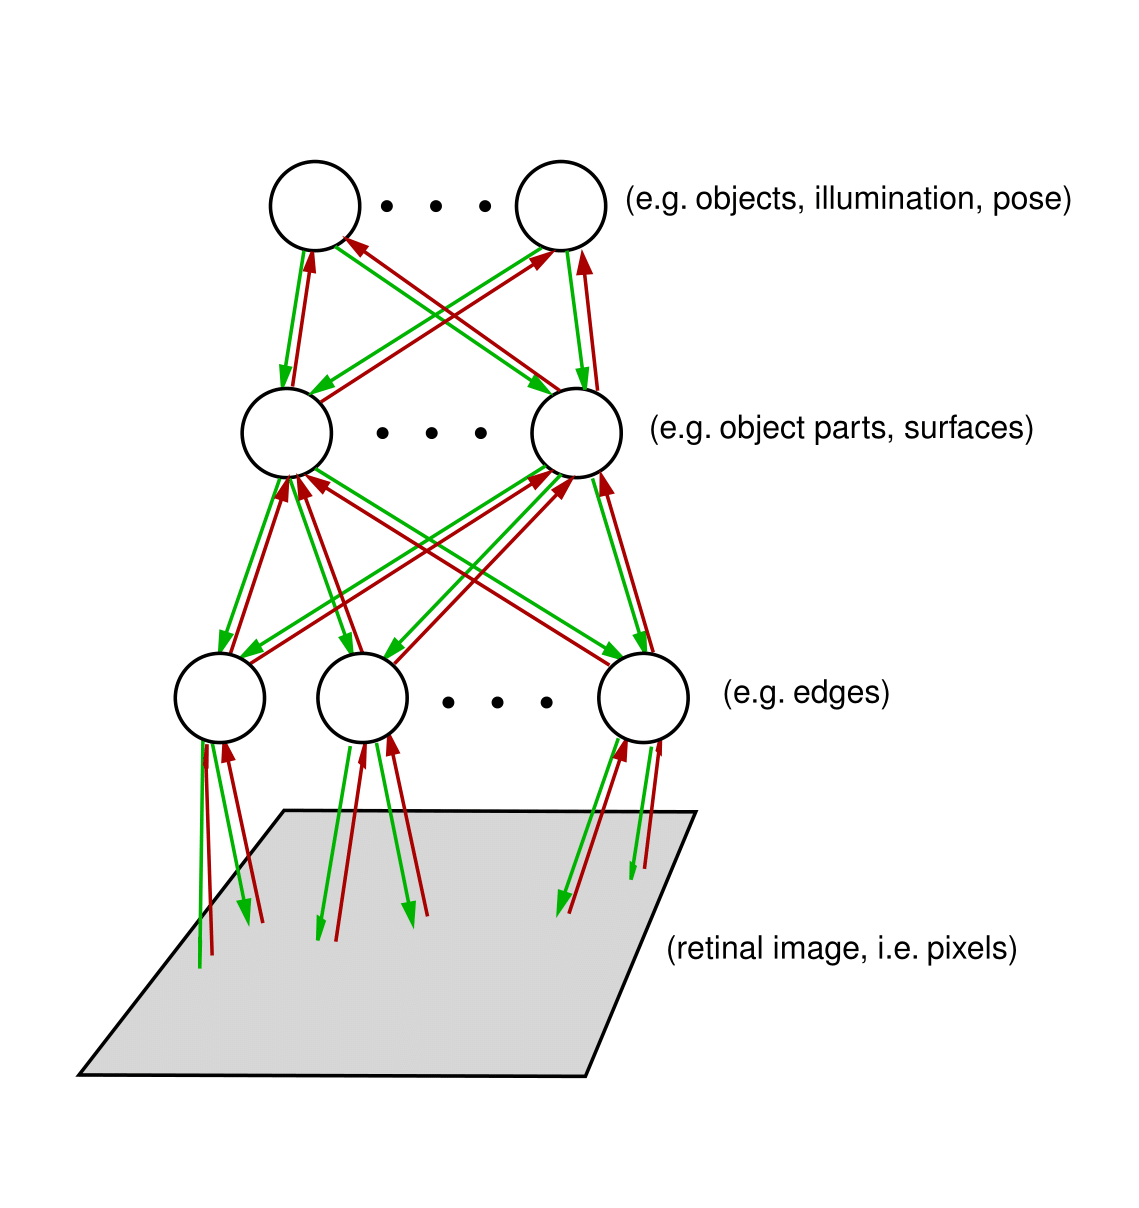
\includegraphics[width=0.5\textwidth,natwidth=1139,natheight=1208]{latentvar}
\caption{Illustration of a probabilistic model with latent variables. Green arrows represent the generative process, in which higher-level concepts guide the development of lower-level ones, eventually leading to the generation of each pixel in an image. Red arrows depict inference, in which case the goal it to infer the underlying causes of an obtained input.}
\label{fig:latent-vars}
\end{center}
\end{figure}

\noindent One immediate drawback to using more complicated latent variable models is that evaluating the likelihood turns out to be intractable, as one has to formally consider the probability of the observed datapoint under every possible setting of the latents. More specifically, consider an observable random variable $\boldsymbol{x}$, an unobserved latent $\boldsymbol{z}$, and their joint distribution $p_{\boldsymbol{\theta}}(\boldsymbol{x}, \boldsymbol{z})$, where the vector $\boldsymbol{\theta}$ denotes the parameters of the generative model. Then, using the sum rule of probability, we can express the marginal of $\boldsymbol{x}$ as $p_{\boldsymbol{\theta}}(\boldsymbol{x}) = \int p_{\boldsymbol{\theta}}(\boldsymbol{x}, \boldsymbol{z}) d \boldsymbol{z}$. \\

\noindent Naturally, as we are unable to evaluate the likelihood function, explicit optimization of its monotonic tranform, the log-likelihood, presents difficulties as well. Fortunately, there exists a workaround, which entails optimizing a lower-bound of the log-likelihood instead. By introducing a new distribution $q_{\boldsymbol{\phi}}(\boldsymbol{z} | \boldsymbol{x})$, parameterized by $\boldsymbol{\phi}$, into our framework, we can lower-bound the original likelihood as follows:

\begin{equation}
\begin{gathered}
\log p_{\boldsymbol{\theta}}(\boldsymbol{x}) \stackrel{\text{sum rule}}{=} \\
\log \int p_{\boldsymbol{\theta}}(\boldsymbol{x}, \boldsymbol{z}) d \boldsymbol{z} \stackrel{\text{multiply by identity}}{=} \\ 
\log \int p_{\boldsymbol{\theta}}(\boldsymbol{x}, \boldsymbol{z}) \frac{q_{\boldsymbol{\phi}}(\boldsymbol{z}|\boldsymbol{x})}{q_{\boldsymbol{\phi}}(\boldsymbol{z}|\boldsymbol{x})} d \boldsymbol{z} \stackrel{\text{Jensen's inequality}}{\geq} \\ 
\int q_{\boldsymbol{\phi}}(\boldsymbol{z}|\boldsymbol{x}) \log \frac{p_{\boldsymbol{\theta}}(\boldsymbol{x}, \boldsymbol{z})}{q_{\boldsymbol{\phi}}(\boldsymbol{z}|\boldsymbol{x})} d \boldsymbol{z} =: \mathcal{L}(\boldsymbol{x}; \boldsymbol{\theta}, \boldsymbol{\phi}). \\
\end{gathered}
\label{eq:free-energy}
\end{equation} \\

\noindent To see that this lower bound could indeed make the optimization problem easier, it helps to write it in two different forms. The first form illustrates that the lower bound can be written as the expected log-joint under the approximate posterior, plus an additive entropy term that does not depend on the parameters of the generative model:

\begin{equation}
\begin{gathered}
\mathcal{L}(\boldsymbol{x}; \boldsymbol{\theta}, \boldsymbol{\phi}) = \\
\int q_{\boldsymbol{\phi}} (\boldsymbol{z}|\boldsymbol{x}) \log p_{\boldsymbol{\theta}}(\boldsymbol{x}, \boldsymbol{z}) d \boldsymbol{z} - \int q_{\boldsymbol{\phi}} (\boldsymbol{z}|\boldsymbol{x}) \log (\boldsymbol{z}|\boldsymbol{x}) d \boldsymbol{z} = \\
\mathbb{E}_{\boldsymbol{z} \sim q_{\boldsymbol{\phi}}(\boldsymbol{z}|\boldsymbol{x})} \big[ \log p_{\boldsymbol{\theta}}(\boldsymbol{x}, \boldsymbol{z}) \big] + \mathcal{H}(q_{\boldsymbol{\phi}} \big(\boldsymbol{z}|\boldsymbol{x}) \big).
\end{gathered}
\label{eq:free-energy-entropy}
\end{equation} \\

\noindent The second form reveals that the free energy is nothing more than the original log-likelihood that we are lower-bounding, minus an additional penalty term which increases the gap between the bound and the log-likelihood in proportion to the distance between the approximate posterior and the real posterior, as measured by Kullback-Leibler divergence:

\begin{equation}
\begin{gathered}
\mathcal{L}(\boldsymbol{x}; \boldsymbol{\theta}, \boldsymbol{\phi}) = \\
\int q_{\boldsymbol{\phi}}(\boldsymbol{z}|\boldsymbol{x}) \log \frac{p_{\boldsymbol{\theta}}(\boldsymbol{z}|\boldsymbol{x})p_{\boldsymbol{\theta}}(\boldsymbol{x})}{q_{\boldsymbol{\phi}}(\boldsymbol{z}|\boldsymbol{x})} d \boldsymbol{z} = \\
\int q_{\boldsymbol{\phi}}(\boldsymbol{z}|\boldsymbol{x}) \log p_{\boldsymbol{\theta}} (\boldsymbol{x}) + \int q_{\boldsymbol{\phi}}(\boldsymbol{z}|\boldsymbol{x}) \log \frac{p_{\boldsymbol{\theta}}(\boldsymbol{z}|\boldsymbol{x})}{q_{\boldsymbol{\phi}}(\boldsymbol{z}|\boldsymbol{x})} d \boldsymbol{z} = \\
\log p_{\boldsymbol{\theta}} (\boldsymbol{x}) - \text{KL}\big(q_{\boldsymbol{\phi}}(\boldsymbol{z}|\boldsymbol{x}) || p_{\boldsymbol{\theta}}(\boldsymbol{z}|\boldsymbol{x}) \big).
\end{gathered}
\label{eq:free-energy-kl}
\end{equation} \\

\noindent Having laid out the two forms of the lower bound, one should notice that in equation \ref{eq:free-energy-entropy}, only the first term depends on the generative parameters $\boldsymbol{\theta}$, while in equation \ref{eq:free-energy-kl}, the parameters of the approximate posterior feature only in the divergence term. This observation suggests a coordinate-wise optimization scheme where we take turns optimizing $\boldsymbol{\theta}$ and $\boldsymbol{\phi}$, leading us to the well-known Expectation-Maximization (EM) algorithm \cite{missing-data}. This approach is applicable when we have analytically tractable forms for the expectation of the log-joint, as well as for the true posterior under the current generative parameters $\boldsymbol{\theta}$.

\noindent What makes EM particularly appealing is that each full step of the algorithm either increases the log-likelihood, or the algorithm has converged to the latter's local maximum. From equation \ref{eq:free-energy-kl}, we see that free energy is maximized with respect to $\boldsymbol{\phi}$ when the KL vanishes (as it is always non-negative), which is accomplished when the approximate posterior \footnote{Note that it is important to distinguish between the best-guess parameters that we are working with when carrying out the optimization scheme, and the maximum-likelihood parameters. Our objective is to find the latter, but we are always operating with an estimated set of parameters. When referring to the \textit{true} posterior, we are not implying that we have access to the true, maximum-likelihood parameters, but the "true" form of the posterior, i.e. $p(x|z)$ as opposed to $q(x|z)$.}is set equal to the true posterior. After that, the lower bound is equal to the log-likelihood (under the current best-guess parameters). Since the next step, maximization with respect to $\boldsymbol{\theta}$ can not decrease the free energy, we observe from equation \ref{eq:free-energy-kl} that the log-likelihood can also not decarease, again due to the non-negativity of KL divergences. \\

\noindent Some of the latent variable models that have tractable expected log-joints and posteriors, yielding EM an appropriate tool for learning their parameters, include factor analysis, mixture of Gaussians, hidden markov models, and linear gaussian state-space models. However, often we are interested in using more complicated graphical models, particularly ones where continuous priors and conditionals have non-linear interactions. Assuming that we have the required derivatives of the lower bound in hand, one solutions would be to optimize the bound directly using regular gradient-based methods. Keeping in mind that this approach is usually inferior to EM, as it loses the theoretical guarantees the latter provides, it is often the method of choice for handling models with intractabilities. A concrete example of such an approach is the variational autoencoder, the topic of the next section.

\section{Variational autoencoders}

As already alluded to in the previous section, the variational autoencoder, introduced by Kingma and Welling \cite{vae}, is a model that optimizes the lower bound of the log-likelihood (equation \ref{eq:free-energy}) using a gradient-based optimization scheme. The form of the lower bound that it is explicitly working with is as follows:

\begin{equation}
\begin{gathered}
\mathcal{L}(\boldsymbol{x}; \boldsymbol{\theta}, \boldsymbol{\phi}) = \\
\int q_{\boldsymbol{\phi}}(\boldsymbol{z}|\boldsymbol{x}) \log \frac{p_{\boldsymbol{\theta}}(\boldsymbol{x} | \boldsymbol{z}) p_{\boldsymbol{\theta}}(\boldsymbol{z})}{q_{\boldsymbol{\phi}}(\boldsymbol{z}|\boldsymbol{x})} d \boldsymbol{z} = \\ 
\int q_{\boldsymbol{\phi}}(\boldsymbol{z}|\boldsymbol{x}) \log p_{\boldsymbol{\theta}}(\boldsymbol{x} | \boldsymbol{z}) d \boldsymbol{z} + \int q_{\boldsymbol{\phi}}(\boldsymbol{z}|\boldsymbol{x}) \log \frac{p_{\boldsymbol{\theta}}(\boldsymbol{z})}{q_{\boldsymbol{\phi}}(\boldsymbol{z}|\boldsymbol{x})} d \boldsymbol{z}  = \\
\int q_{\boldsymbol{\phi}}(\boldsymbol{z}|\boldsymbol{x}) \log p_{\boldsymbol{\theta}}(\boldsymbol{x} | \boldsymbol{z}) d \boldsymbol{z} - \text{KL}(q_{\boldsymbol{\phi}}(\boldsymbol{z}|\boldsymbol{x}) || p_{\boldsymbol{\theta}}(\boldsymbol{z})) = \\
\mathbb{E}_{\boldsymbol{z} \sim q_{\boldsymbol{\phi}}(\boldsymbol{z}|\boldsymbol{x})} \big[ \log p_{\boldsymbol{\theta}} (\boldsymbol{x} | \boldsymbol{z}) \big] - \text{KL}(q_{\boldsymbol{\phi}}(\boldsymbol{z}|\boldsymbol{x}) || p_{\boldsymbol{\theta}}(\boldsymbol{z})) \simeq \\
\frac{1}{L} \sum_{l=1}^L \log p_{\boldsymbol{\theta}} (\boldsymbol{x} | \boldsymbol{z}^{(l)}) - \text{KL}(q_{\boldsymbol{\phi}}(\boldsymbol{z}|\boldsymbol{x}) || p_{\boldsymbol{\theta}}(\boldsymbol{z})), \quad \text{where } \boldsymbol{z}^{(l)} \sim q_{\boldsymbol{\phi}}(\boldsymbol{z}^{(l)} | \boldsymbol{x}),
\end{gathered}
\label{eq:vae-lb}
\end{equation} \\

\noindent where the first term of the last line is a Monte-Carlo estimate of the expectation above. The KL divergence is left as-is, because as we will soon see, for common distributions, it can be calculated analytically. In general, however, this term can also be estimated by a finite set of samples as well. \\

\noindent An immediate problem that presents itself is that sampling directly from the approximate posterior is not a continuous operation. This presents a problem, as we need the gradient of the Monte-Carlo estimate of the lower bound with respect to $\boldsymbol{\phi}$ for optimization. In principle, the necessary gradients could be estimated using the score function estimator, an ubiquitious method in the reinforcement learning literature \cite{Williams1992}:

\begin{equation}
\begin{gathered}
\nabla_{\boldsymbol{\phi}} \mathbb{E}_{\boldsymbol{z} \sim q_{\boldsymbol{\phi}}(\boldsymbol{z}|\boldsymbol{x})} \big[ \log p_{\boldsymbol{\theta}} (\boldsymbol{x} | \boldsymbol{z}) \big] = \\
\int \nabla_{\boldsymbol{\phi}} q_{\boldsymbol{\phi}}(\boldsymbol{z}|\boldsymbol{x}) \log p_{\boldsymbol{\theta}}(\boldsymbol{x} | \boldsymbol{z}) d \boldsymbol{z} \stackrel{\text{multiply by identity}}{=} \\
\int \frac{q_{\boldsymbol{\phi}}(\boldsymbol{z}|\boldsymbol{x})}{q_{\boldsymbol{\phi}}(\boldsymbol{z}|\boldsymbol{x})} \nabla_{\boldsymbol{\phi}} q_{\boldsymbol{\phi}}(\boldsymbol{z}|\boldsymbol{x}) \log p_{\boldsymbol{\theta}}(\boldsymbol{x} | \boldsymbol{z}) d \boldsymbol{z} \stackrel{\text{derivative of log}}{=} \\
\int q_{\boldsymbol{\phi}}(\boldsymbol{z}|\boldsymbol{x}) \nabla_{\boldsymbol{\phi}} \log q_{\boldsymbol{\phi}}(\boldsymbol{z}|\boldsymbol{x}) \log p_{\boldsymbol{\theta}}(\boldsymbol{x} | \boldsymbol{z}) d \boldsymbol{z} = \\
\mathbb{E}_{\boldsymbol{z} \sim q_{\boldsymbol{\phi}}(\boldsymbol{z}|\boldsymbol{x})} \big[ \nabla_{\boldsymbol{\phi}} \log q_{\boldsymbol{\phi}}(\boldsymbol{z}|\boldsymbol{x}) \log p_{\boldsymbol{\theta}}(\boldsymbol{x} | \boldsymbol{z}) \big] \simeq \\
\frac{1}{L} \sum_{l=1}^L \nabla_{\boldsymbol{\phi}} \log q_{\boldsymbol{\phi}}(\boldsymbol{z}|\boldsymbol{x}) \log p_{\boldsymbol{\theta}}(\boldsymbol{x} | \boldsymbol{z}), \quad \text{where } \boldsymbol{z}^{(l)} \sim q_{\boldsymbol{\phi}}(\boldsymbol{z}^{(l)} | \boldsymbol{x}).
\end{gathered}
\end{equation} \\

\noindent Unfortunately, due to its generality, the preceding estimator has a very high variance, rendering it impractical for the purposes of generative modelling.

\todo{Talk about the reparameterization trick}

\section{Disentangled representations}

\section{Adversarial examples}
\chapter{Methods}

\chapter{Results}

\begin{center}
{\tiny
  \begin{tabular}{|c|c|c|c|c|c|c|c|c|c|c|}
  \hline
  \textbf{Source} & \textbf{0} & \textbf{1} & \textbf{2} & \textbf{3} & \textbf{4} & \textbf{5} & \textbf{6} & \textbf{7} & \textbf{8} & \textbf{9}  \\ \hline
  \textbf{AS ignore-target} & 8.80\% & 82.58\% & 20.46\% & 16.52\% & 32.74\% & 43.58\% & 38.25\% & 40.10\% & 18.68\% & 64.22\% \\ \hline
  \textbf{AS target} & 3.25\% & 34.05\% & 5.59\% & 6.15\% & 12.26\% & 10.88\% & 13.21\% & 11.85\% & 8.52\% & 19.30\% \\ \hline
  \end{tabular}
}
\captionof{table}{Disentangled marginals}
\end{center}

\begin{center}
{\tiny
  \begin{tabular}{|c|c|c|c|c|c|c|c|c|c|c|}
  \hline
  \textbf{Source} & \textbf{0} & \textbf{1} & \textbf{2} & \textbf{3} & \textbf{4} & \textbf{5} & \textbf{6} & \textbf{7} & \textbf{8} & \textbf{9}  \\ \hline
  \textbf{AS ignore-target} & 5.87\% & 63.87\% & 11.49\% & 12.52\% & 64.10\% & 36.82\% & 26.99\% & 39.75\% & 16.21\% & 19.36\% \\ \hline
  \textbf{AS target} & 1.88\% & 28.19\% & 3.24\% & 4.33\% & 13.48\% & 10.19\% & 8.81\% & 7.71\% & 5.71\% & 8.22\% \\ \hline
  \end{tabular}
}
\captionof{table}{Entangled marginals}
\end{center}

\begin{center}
{\tiny
  \begin{tabular}{|c|c|c|c|c|c|c|c|c|c|c|}
  \hline
  \textbf{Source} & \textbf{0} & \textbf{1} & \textbf{2} & \textbf{3} & \textbf{4} & \textbf{5} & \textbf{6} & \textbf{7} & \textbf{8} & \textbf{9}  \\ \hline
  \textbf{AS ignore-target} & 3.21\% & 60.25\% & 7.43\% & 10.57\% & 53.79\% & 35.07\% & 25.06\% & 18.52\% & 23.28\% & 33.15\% \\ \hline
  \textbf{AS target} & 0.86\% & 23.52\% & 1.46\% & 2.88\% & 10.88\% & 9.28\% & 6.34\% & 4.24\% & 8.24\% & 12.08\% \\ \hline
  \end{tabular}
}
\captionof{table}{Entangled weight decay marginals}
\end{center}

\chapter{Conclusion}

\chapter{Appendix}


\begin{center}
{\tiny
  \begin{tabular}{|c|c|c|c|c|c|c|c|c|c|c|}
  \cline{1-11}
  \multirow{2}{*}{\textbf{Source}}
  & \multicolumn{10}{ c| }{\textbf{Targets}}  \\ \cline {2-11}
  & \textbf{0} & \textbf{1} & \textbf{2} & \textbf{3} & \textbf{4} & \textbf{5} & \textbf{6} & \textbf{7} & \textbf{8} & \textbf{9}  \\ \hline
  \textbf{0} & - & \makecell{7.02\% \\ (0.00\%)} & \makecell{9.80\% \\ (5.74\%)} & \makecell{7.64\% \\ (4.29\%)} & \makecell{9.62\% \\ (1.88\%)} & \makecell{11.60\% \\ (5.86\%)} & \makecell{8.63\% \\ (5.43\%)} & \makecell{6.68\% \\ (0.10\%)} & \makecell{9.45\% \\ (5.67\%)} & \makecell{8.80\% \\ (0.31\%)} \\ \hline
  \textbf{1} & \makecell{99.16\% \\ (0.00\%)} & - & \makecell{98.41\% \\ (93.66\%)} & \makecell{95.32\% \\ (4.48\%)} & \makecell{74.11\% \\ (44.89\%)} & \makecell{94.50\% \\ (10.42\%)} & \makecell{98.07\% \\ (26.55\%)} & \makecell{23.25\% \\ (13.57\%)} & \makecell{95.06\% \\ (73.08\%)} & \makecell{65.31\% \\ (39.78\%)} \\ \hline
  \textbf{2} & \makecell{8.75\% \\ (1.01\%)} & \makecell{23.32\% \\ (0.43\%)} & - & \makecell{16.29\% \\ (5.93\%)} & \makecell{25.75\% \\ (4.79\%)} & \makecell{23.54\% \\ (1.58\%)} & \makecell{6.86\% \\ (2.29\%)} & \makecell{25.03\% \\ (12.78\%)} & \makecell{26.04\% \\ (21.08\%)} & \makecell{28.59\% \\ (0.44\%)} \\ \hline
  \textbf{3} & \makecell{3.23\% \\ (0.58\%)} & \makecell{19.82\% \\ (0.34\%)} & \makecell{16.09\% \\ (12.37\%)} & - & \makecell{19.91\% \\ (0.81\%)} & \makecell{16.50\% \\ (14.61\%)} & \makecell{12.22\% \\ (1.90\%)} & \makecell{19.39\% \\ (1.70\%)} & \makecell{23.23\% \\ (18.40\%)} & \makecell{18.29\% \\ (4.60\%)} \\ \hline
  \textbf{4} & \makecell{24.32\% \\ (0.37\%)} & \makecell{42.75\% \\ (0.49\%)} & \makecell{38.03\% \\ (24.18\%)} & \makecell{28.12\% \\ (6.60\%)} & - & \makecell{22.59\% \\ (4.10\%)} & \makecell{19.77\% \\ (11.01\%)} & \makecell{50.60\% \\ (7.13\%)} & \makecell{34.12\% \\ (25.46\%)} & \makecell{34.38\% \\ (30.99\%)} \\ \hline
  \textbf{5} & \makecell{46.78\% \\ (3.42\%)} & \makecell{45.72\% \\ (0.92\%)} & \makecell{64.34\% \\ (8.55\%)} & \makecell{34.30\% \\ (26.49\%)} & \makecell{30.23\% \\ (7.59\%)} & - & \makecell{51.84\% \\ (11.15\%)} & \makecell{41.29\% \\ (1.72\%)} & \makecell{49.41\% \\ (31.49\%)} & \makecell{28.35\% \\ (6.56\%)} \\ \hline
  \textbf{6} & \makecell{28.31\% \\ (6.89\%)} & \makecell{34.79\% \\ (2.51\%)} & \makecell{41.54\% \\ (32.64\%)} & \makecell{37.96\% \\ (6.35\%)} & \makecell{37.31\% \\ (22.98\%)} & \makecell{32.55\% \\ (10.34\%)} & - & \makecell{39.48\% \\ (2.40\%)} & \makecell{49.02\% \\ (28.82\%)} & \makecell{43.31\% \\ (5.98\%)} \\ \hline
  \textbf{7} & \makecell{46.96\% \\ (2.03\%)} & \makecell{3.51\% \\ (0.11\%)} & \makecell{38.03\% \\ (23.94\%)} & \makecell{47.00\% \\ (2.54\%)} & \makecell{37.46\% \\ (5.23\%)} & \makecell{50.65\% \\ (5.63\%)} & \makecell{43.61\% \\ (0.60\%)} & - & \makecell{51.19\% \\ (29.52\%)} & \makecell{42.53\% \\ (37.01\%)} \\ \hline
  \textbf{8} & \makecell{26.31\% \\ (0.91\%)} & \makecell{13.01\% \\ (1.47\%)} & \makecell{31.15\% \\ (25.29\%)} & \makecell{23.31\% \\ (13.83\%)} & \makecell{11.44\% \\ (5.95\%)} & \makecell{20.38\% \\ (11.75\%)} & \makecell{22.88\% \\ (6.85\%)} & \makecell{10.97\% \\ (5.37\%)} & - & \makecell{8.69\% \\ (5.26\%)} \\ \hline
  \textbf{9} & \makecell{80.48\% \\ (0.80\%)} & \makecell{40.13\% \\ (1.77\%)} & \makecell{79.96\% \\ (5.46\%)} & \makecell{81.37\% \\ (22.60\%)} & \makecell{38.78\% \\ (36.85\%)} & \makecell{74.43\% \\ (24.06\%)} & \makecell{75.00\% \\ (3.90\%)} & \makecell{27.42\% \\ (20.96\%)} & \makecell{80.37\% \\ (57.27\%)} & - \\ \hline
     \end{tabular}
}
\captionof{table}{Disentangled}
\end{center}


\begin{center}
{\tiny
  \begin{tabular}{|c|c|c|c|c|c|c|c|c|c|c|}
  \cline{1-11}
  \multirow{2}{*}{\textbf{Source}}
  & \multicolumn{10}{ c| }{\textbf{Targets}}  \\ \cline {2-11}
  & \textbf{0} & \textbf{1} & \textbf{2} & \textbf{3} & \textbf{4} & \textbf{5} & \textbf{6} & \textbf{7} & \textbf{8} & \textbf{9}  \\ \hline
  \textbf{0} & - & \makecell{3.33\% \\ (0.00\%)} & \makecell{8.67\% \\ (2.82\%)} & \makecell{6.93\% \\ (2.10\%)} & \makecell{6.33\% \\ (0.10\%)} & \makecell{5.49\% \\ (1.83\%)} & \makecell{4.80\% \\ (2.24\%)} & \makecell{3.96\% \\ (0.00\%)} & \makecell{9.04\% \\ (5.99\%)} & \makecell{4.28\% \\ (1.88\%)} \\ \hline
  \textbf{1} & \makecell{60.50\% \\ (0.21\%)} & - & \makecell{75.57\% \\ (51.43\%)} & \makecell{71.26\% \\ (40.99\%)} & \makecell{61.83\% \\ (24.38\%)} & \makecell{66.78\% \\ (14.38\%)} & \makecell{50.48\% \\ (18.72\%)} & \makecell{62.99\% \\ (28.26\%)} & \makecell{74.19\% \\ (56.95\%)} & \makecell{51.22\% \\ (18.36\%)} \\ \hline
  \textbf{2} & \makecell{13.65\% \\ (1.53\%)} & \makecell{4.04\% \\ (0.10\%)} & - & \makecell{14.32\% \\ (11.05\%)} & \makecell{10.55\% \\ (0.66\%)} & \makecell{13.62\% \\ (0.24\%)} & \makecell{10.94\% \\ (1.80\%)} & \makecell{8.49\% \\ (1.15\%)} & \makecell{16.67\% \\ (11.00\%)} & \makecell{11.15\% \\ (1.61\%)} \\ \hline
  \textbf{3} & \makecell{8.89\% \\ (0.56\%)} & \makecell{5.50\% \\ (0.11\%)} & \makecell{8.79\% \\ (4.45\%)} & - & \makecell{21.85\% \\ (0.33\%)} & \makecell{14.23\% \\ (10.80\%)} & \makecell{12.49\% \\ (0.57\%)} & \makecell{5.60\% \\ (0.54\%)} & \makecell{26.02\% \\ (19.91\%)} & \makecell{9.30\% \\ (1.73\%)} \\ \hline
  \textbf{4} & \makecell{70.34\% \\ (2.76\%)} & \makecell{42.32\% \\ (0.33\%)} & \makecell{68.65\% \\ (9.35\%)} & \makecell{89.19\% \\ (10.26\%)} & - & \makecell{77.03\% \\ (4.84\%)} & \makecell{23.84\% \\ (3.95\%)} & \makecell{71.62\% \\ (4.77\%)} & \makecell{75.28\% \\ (30.85\%)} & \makecell{58.65\% \\ (54.19\%)} \\ \hline
  \textbf{5} & \makecell{34.34\% \\ (2.67\%)} & \makecell{22.46\% \\ (0.25\%)} & \makecell{47.30\% \\ (4.90\%)} & \makecell{36.06\% \\ (24.04\%)} & \makecell{36.29\% \\ (0.37\%)} & - & \makecell{25.98\% \\ (6.62\%)} & \makecell{36.05\% \\ (0.37\%)} & \makecell{57.67\% \\ (43.56\%)} & \makecell{35.26\% \\ (8.97\%)} \\ \hline
  \textbf{6} & \makecell{23.43\% \\ (16.49\%)} & \makecell{7.59\% \\ (0.22\%)} & \makecell{29.71\% \\ (7.35\%)} & \makecell{42.27\% \\ (8.71\%)} & \makecell{14.30\% \\ (6.60\%)} & \makecell{24.36\% \\ (11.59\%)} & - & \makecell{37.38\% \\ (0.00\%)} & \makecell{41.28\% \\ (25.68\%)} & \makecell{22.61\% \\ (2.61\%)} \\ \hline
  \textbf{7} & \makecell{33.44\% \\ (1.55\%)} & \makecell{24.53\% \\ (0.32\%)} & \makecell{29.70\% \\ (6.77\%)} & \makecell{32.36\% \\ (15.10\%)} & \makecell{53.05\% \\ (6.09\%)} & \makecell{39.25\% \\ (1.22\%)} & \makecell{55.95\% \\ (0.45\%)} & - & \makecell{54.59\% \\ (8.72\%)} & \makecell{34.88\% \\ (29.17\%)} \\ \hline
  \textbf{8} & \makecell{13.36\% \\ (1.03\%)} & \makecell{7.41\% \\ (0.11\%)} & \makecell{19.88\% \\ (8.44\%)} & \makecell{34.31\% \\ (28.09\%)} & \makecell{10.35\% \\ (1.25\%)} & \makecell{22.35\% \\ (5.74\%)} & \makecell{10.06\% \\ (1.73\%)} & \makecell{18.65\% \\ (0.80\%)} & - & \makecell{9.49\% \\ (4.23\%)} \\ \hline
  \textbf{9} & \makecell{8.41\% \\ (1.44\%)} & \makecell{6.57\% \\ (0.32\%)} & \makecell{32.33\% \\ (1.72\%)} & \makecell{36.72\% \\ (20.34\%)} & \makecell{14.97\% \\ (11.20\%)} & \makecell{24.48\% \\ (7.67\%)} & \makecell{7.81\% \\ (0.23\%)} & \makecell{12.81\% \\ (6.35\%)} & \makecell{30.10\% \\ (24.70\%)} & - \\ \hline
  \end{tabular}
}
\captionof{table}{Entangled}
\end{center}

\begin{center}
{\tiny
  \begin{tabular}{|c|c|c|c|c|c|c|c|c|c|c|}
  \cline{1-11}
  \multirow{2}{*}{\textbf{Source}}
  & \multicolumn{10}{ c| }{\textbf{Targets}}  \\ \cline {2-11}
  & \textbf{0} & \textbf{1} & \textbf{2} & \textbf{3} & \textbf{4} & \textbf{5} & \textbf{6} & \textbf{7} & \textbf{8} & \textbf{9}  \\ \hline
  \textbf{0} & - & \makecell{2.22\% \\ (0.00\%)} & \makecell{5.60\% \\ (1.27\%)} & \makecell{4.95\% \\ (1.90\%)} & \makecell{2.11\% \\ (0.00\%)} & \makecell{4.15\% \\ (0.92\%)} & \makecell{2.05\% \\ (1.08\%)} & \makecell{1.68\% \\ (0.00\%)} & \makecell{3.74\% \\ (2.14\%)} & \makecell{2.40\% \\ (0.42\%)} \\ \hline
\textbf{1} & \makecell{70.15\% \\ (2.19\%)} & - & \makecell{75.69\% \\ (59.23\%)} & \makecell{65.31\% \\ (24.92\%)} & \makecell{39.46\% \\ (3.43\%)} & \makecell{56.55\% \\ (8.51\%)} & \makecell{39.42\% \\ (16.67\%)} & \makecell{64.58\% \\ (50.20\%)} & \makecell{78.83\% \\ (36.27\%)} & \makecell{52.23\% \\ (10.24\%)} \\ \hline
\textbf{2} & \makecell{8.79\% \\ (2.05\%)} & \makecell{4.53\% \\ (0.11\%)} & - & \makecell{6.61\% \\ (3.41\%)} & \makecell{6.69\% \\ (0.68\%)} & \makecell{9.53\% \\ (0.12\%)} & \makecell{8.34\% \\ (1.16\%)} & \makecell{7.46\% \\ (1.71\%)} & \makecell{7.74\% \\ (3.35\%)} & \makecell{7.19\% \\ (0.55\%)} \\ \hline
\textbf{3} & \makecell{9.45\% \\ (1.08\%)} & \makecell{5.85\% \\ (0.11\%)} & \makecell{9.47\% \\ (6.47\%)} & - & \makecell{14.82\% \\ (0.00\%)} & \makecell{14.01\% \\ (9.51\%)} & \makecell{12.02\% \\ (0.74\%)} & \makecell{8.44\% \\ (2.43\%)} & \makecell{9.60\% \\ (4.32\%)} & \makecell{11.51\% \\ (1.27\%)} \\ \hline
\textbf{4} & \makecell{54.66\% \\ (2.64\%)} & \makecell{28.52\% \\ (1.62\%)} & \makecell{57.04\% \\ (17.21\%)} & \makecell{73.44\% \\ (5.99\%)} & - & \makecell{74.53\% \\ (2.28\%)} & \makecell{25.22\% \\ (3.95\%)} & \makecell{60.29\% \\ (12.50\%)} & \makecell{64.06\% \\ (10.97\%)} & \makecell{46.33\% \\ (40.72\%)} \\ \hline
\textbf{5} & \makecell{40.51\% \\ (13.69\%)} & \makecell{20.58\% \\ (1.37\%)} & \makecell{42.05\% \\ (3.56\%)} & \makecell{32.15\% \\ (19.35\%)} & \makecell{39.34\% \\ (0.69\%)} & - & \makecell{33.92\% \\ (8.72\%)} & \makecell{34.32\% \\ (6.89\%)} & \makecell{37.85\% \\ (22.15\%)} & \makecell{34.92\% \\ (7.09\%)} \\ \hline
\textbf{6} & \makecell{18.98\% \\ (14.46\%)} & \makecell{8.28\% \\ (1.20\%)} & \makecell{35.20\% \\ (11.62\%)} & \makecell{33.00\% \\ (3.51\%)} & \makecell{15.51\% \\ (4.84\%)} & \makecell{19.98\% \\ (5.52\%)} & - & \makecell{31.84\% \\ (0.33\%)} & \makecell{39.14\% \\ (14.33\%)} & \makecell{23.60\% \\ (1.21\%)} \\ \hline
\textbf{7} & \makecell{13.27\% \\ (1.72\%)} & \makecell{7.84\% \\ (1.18\%)} & \makecell{21.82\% \\ (11.18\%)} & \makecell{18.72\% \\ (8.08\%)} & \makecell{19.12\% \\ (1.04\%)} & \makecell{18.45\% \\ (1.12\%)} & \makecell{23.76\% \\ (0.12\%)} & - & \makecell{29.38\% \\ (3.72\%)} & \makecell{14.30\% \\ (10.01\%)} \\ \hline
\textbf{8} & \makecell{19.11\% \\ (4.97\%)} & \makecell{15.19\% \\ (1.42\%)} & \makecell{37.68\% \\ (28.19\%)} & \makecell{33.12\% \\ (18.57\%)} & \makecell{16.25\% \\ (0.40\%)} & \makecell{17.43\% \\ (3.86\%)} & \makecell{25.20\% \\ (4.96\%)} & \makecell{30.09\% \\ (6.18\%)} & - & \makecell{15.43\% \\ (5.58\%)} \\ \hline
\textbf{9} & \makecell{25.66\% \\ (2.89\%)} & \makecell{16.65\% \\ (1.50\%)} & \makecell{49.94\% \\ (11.74\%)} & \makecell{56.67\% \\ (22.12\%)} & \makecell{13.68\% \\ (6.49\%)} & \makecell{37.21\% \\ (8.22\%)} & \makecell{21.00\% \\ (0.49\%)} & \makecell{38.96\% \\ (35.61\%)} & \makecell{38.54\% \\ (19.69\%)} & - \\ \hline
  \end{tabular}
}
\captionof{table}{Entangled with weight decay}
\end{center}


\newpage
\bibliographystyle{plain}
\bibliography{report}{}

\end{document}

